%==============================================================================
%  FINAL PROJECT PAPER  (IEEE Conference format)
%  Category B — AI-Agent Code Optimization
%  Parallel Programming, Spring 2026
%==============================================================================
\documentclass[conference]{IEEEtran}
\IEEEoverridecommandlockouts

\usepackage{cite}
\usepackage{amsmath,amssymb,amsfonts}
\usepackage{algorithmic}
\usepackage{graphicx}
\usepackage{textcomp}
\usepackage{xcolor}
\usepackage{listings}
\usepackage{url}
\usepackage{booktabs}
\usepackage{multirow}
\usepackage[hidelinks]{hyperref}

\newcommand{\mainbodyendpage}{?}
\AtEndDocument{%
  \typeout{====================================================}%
  \typeout{[PAGE BUDGET] Main body + references end on page \mainbodyendpage\space (limit: 6).}%
  \typeout{====================================================}%
}

\lstset{
  basicstyle=\ttfamily\footnotesize,
  breaklines=true,
  frame=single,
  columns=fullflexible,
  showstringspaces=false,
  keepspaces=true,
  xleftmargin=0.5em
}

\begin{document}

\title{Can LLMs Parallelize and Optimize CUDA?\\
A Study with the Rodinia Benchmark Suite\\
{\footnotesize Final Project --- Parallel Programming, Spring 2026}}

\author{%
\IEEEauthorblockN{Cheng-Jui Lee}
\IEEEauthorblockA{r14922017 \\ CSIE, NTU \\ r14922017@csie.ntu.edu.tw}%
\and
\IEEEauthorblockN{Chun-Chieh Yeh}
\IEEEauthorblockA{r13922156 \\ CSIE, NTU \\ r13922156@csie.ntu.edu.tw}
}

\maketitle

\begin{abstract}
We systematically evaluate whether state-of-the-art large language models (LLMs)
can blindly parallelize and optimize CUDA kernels from the Rodinia benchmark
suite. Three models---Claude Opus, Sonnet, and Haiku---are tested on eight
benchmarks in a two-phase protocol: Phase~1 requires a naive global-memory CUDA
port without profiling information; Phase~2 unlocks hardware optimizations with
iterative nsys profiling feedback. We design an automated evaluation harness that
builds, verifies correctness against a serial golden output, and measures GPU
kernel time. Across the eight benchmarks, the dominant factor in the outcome is
the benchmark's parallelism structure rather than the model tier: on memory- and
launch-bound workloads every model converges to the same hardware ceiling, while
on benchmarks that stress CUDA execution-model details correctness tracks model
capability. Opus is the most reliable, producing correct code on all eight;
Sonnet is accurate in Phase~1 but frequently introduces bugs during Phase~2
optimization; Haiku is the least stable, producing no correct version on two of
the eight. For compute-bound workloads, AI-generated CUDA reaches two to three
orders of magnitude of speedup over serial (up to 2891$\times$) and matches or
exceeds the original Rodinia hand-tuned CUDA on every benchmark we could compare
directly. We further show
that harness design---particularly the revert-to-best iteration policy and the
diagnoser stopping criteria---critically affects whether models can compound
optimization gains across rounds.
\end{abstract}

\begin{IEEEkeywords}
CUDA, LLM code generation, GPU optimization, Rodinia benchmark, parallel programming
\end{IEEEkeywords}

\vspace{0.5em}
\noindent\fbox{\parbox{0.97\columnwidth}{\textbf{Project Category:}\quad
$\square$~\textbf{A} (Self-chosen topic)\qquad
$\boxtimes$~\textbf{B} (AI-agent code optimization)}}

%------------------------------------------------------------------------------
\section{Introduction}

Writing high-performance CUDA code is notoriously difficult: a naive parallel
port often runs 100--1000$\times$ slower than a hand-tuned implementation, and
closing that gap requires deep knowledge of GPU memory hierarchy, warp execution,
shared-memory tiling, and occupancy tuning. Large language models (LLMs) have
demonstrated strong general code generation capabilities, raising the question of
whether they can produce \emph{correct and fast} CUDA kernels from a serial
reference alone~\cite{chen2021codex}. This question has direct practical implications: state-of-the-art
frontier models (e.g., Claude Opus) cost roughly 15$\times$ more per token than
lightweight models (e.g., Claude Haiku). If a cheaper model achieves the same GPU
optimization quality, practitioners can save substantially without sacrificing
performance.

We evaluate three Claude models---Opus, Sonnet, and Haiku---on eight benchmarks
from the Rodinia GPU benchmark suite~\cite{che2009rodinia}, using a single
automated harness for all models. Each benchmark is run through a two-phase
protocol: in Phase~1, the model receives only a serial C reference and an
algorithm specification, and must produce a correct CUDA port using global memory
only; in Phase~2, the model iterates for up to four rounds with nsys profiling
feedback (kernel time, transfer times, per-kernel breakdown), and hardware
optimizations such as shared memory and tiling are permitted. Correctness is
verified cell-by-cell against a serial golden output; the primary performance
metric is GPU kernel time measured on a dedicated RTX~3070 to ensure clean timing.

Our results show three distinct patterns. On \textbf{compute-bound} benchmarks
(lavaMD, SRAD, kmeans), Phase~2 optimization yields significant gains (up to
$15\times$ over Phase~1), and model-tier differences emerge in reliability: Opus
produces correct code in all eight benchmarks, while Haiku fails on two. On
\textbf{memory/launch-bound} benchmarks (hotspot, BFS), every model that
produces correct code plateaus at the same hardware ceiling and optimization
headroom is limited. Correctness is the clearest differentiator across models:
Haiku introduces a distinct new bug each round on the harder benchmarks, while
Opus consistently maintains correctness throughout iterative optimization.

%------------------------------------------------------------------------------
\section{Background and Related Work}

\subsection{Rodinia Benchmark Suite}
Rodinia~\cite{che2009rodinia} is a widely-used GPU benchmark collection covering
diverse HPC application patterns. We select eight benchmarks spanning a range of
parallelism structures and memory behaviors:

\begin{itemize}
  \item \textbf{hotspot}: 2D thermal stencil (1024$\times$1024, 1000
        iterations). Each cell depends only on its four neighbors in the
        previous timestep---trivially data-parallel and bandwidth-bound on
        modern GPUs.
  \item \textbf{hotspot3D}: 3D thermal stencil (512$\times$512$\times$8, 100
        iterations). Extends hotspot to a third dimension; also bandwidth-bound.
  \item \textbf{NW}: Needleman--Wunsch global sequence alignment. Cells on the
        same anti-diagonal are independent (wavefront parallelism); diagonal
        width limits occupancy.
  \item \textbf{BFS}: Breadth-first search on a random graph (1M nodes).
        Dominated by host--device transfer and kernel-launch overhead.
  \item \textbf{SRAD}: Speckle Reducing Anisotropic Diffusion, a 2D PDE stencil
        (2048$\times$2048, 100 iterations) with a two-kernel prepare/update
        structure. Compute-bound with a reduction step.
  \item \textbf{lavaMD}: N-body molecular dynamics force calculation
        ($10^3$ boxes, $10^5$ particles). Arithmetic-intensive inner
        force-sum loop; strongly compute-bound.
  \item \textbf{pathfinder}: Row-parallel 1D DP sweep
        (100k columns $\times$ 1000 rows). Each column is independent within a
        row; each cell depends on three cells in the previous row.
  \item \textbf{kmeans}: K-means clustering assign step (65536 points,
        34 features, 5 clusters, 20 iterations). Embarrassingly parallel;
        centroid array (680\,B) fits in constant memory.
\end{itemize}

These eight benchmarks span the full range of GPU parallelism patterns---from
embarrassingly parallel (kmeans) through stencil (hotspot, hotspot3D, SRAD) and
data-dependent dynamic programming (NW, pathfinder) to irregular graph traversal
(BFS) and compute-intensive N-body simulation (lavaMD)---while each admits a
deterministic golden output suitable for automated correctness checking. We draw
on prior characterizations of the suite's parallelism and memory behavior to
reason about which benchmarks have genuine optimization headroom~\cite{che2009rodinia,rodinia2010}.

\subsection{Related Work}
LLM code generation has been benchmarked extensively for general-purpose
programming~\cite{chen2021codex}, but evaluating the \emph{performance}---not
merely correctness---of generated GPU kernels is comparatively underexplored.
Our setup places a profiler in the loop: a diagnoser turns nsys measurements
into targeted feedback, a role similar to automated GPU performance
advisors~\cite{gpa2021}, except the advisor is an LLM agent that both diagnoses
and rewrites the kernel.

%------------------------------------------------------------------------------
\section{Methodology}
\label{sec:method}

\subsection{Two-Phase Protocol}

\textbf{Phase 1 (Blind Naive Port):} The model receives only the serial C
source and an algorithm specification document. It must generate a
correct CUDA port using \emph{global memory only}---no shared memory, tiling,
or hardware-specific optimization. This tests raw parallelization ability
without profiling cues.

\textbf{Phase 2 (Iterative Optimization):} Starting from the Phase~1 result
(or the best correct version so far), the model receives nsys profiling
feedback---kernel time, HtoD/DtoH transfer times, per-kernel breakdown, and
correctness diff---and iterates for up to four rounds including Phase 1. Hardware optimizations
(shared memory, tiling, coalescing, vectorization) are now allowed.

\subsection{Harness Design}

The evaluation harness builds each candidate with \texttt{nvcc}, runs
correctness checks against a serial golden output with configurable
tolerance, profiles with \texttt{nsys}, and checks memory safety with
\texttt{compute-sanitizer}.
The primary metric is nsys GPU kernel time (excluding data transfer), enabling
fair comparison across implementations.

Each benchmark has a \emph{serial reference} derived from the Rodinia OpenMP
version with OpenMP pragmas removed, a deterministic input generator, and a
verified golden output. Float benchmarks disable FMA for correctness builds to
match CPU float32 arithmetic order. Integer benchmarks (BFS, NW, pathfinder,
kmeans) require exact match (zero tolerance).

\subsection{Iteration Policy: Revert-to-Best}

Phase~2 follows a \textbf{revert-to-best policy}: each round always starts from
the model's best correct version so far, not its most recent attempt. A failed
round---wrong output, build error, or performance regression---does not
terminate the loop. Instead, the model is told explicitly what the failed
attempt did and is instructed to try a \emph{different} optimization. This lets
a model recover from an exploratory misstep without discarding the working
baseline it has already reached, and prevents an incorrect intermediate result
from contaminating the context fed to subsequent rounds. If Phase 1 produced no 
correct version, the first Phase-2 round started from the Phase-1 candidate 
together with the mismatch report; once a correct version was found, subsequent 
rounds followed the revert-to-best policy.

The loop terminates on either of two conditions: (a) a hard cap of four Phase~2
rounds, or (b) the diagnoser signals convergence \emph{and} improvement has
flattened. Condition (b) is gated by an \textbf{improvement guard}: if the most
recent round reduced kernel time by $\geq$5\%, the loop overrides the
convergence signal and continues. This prevents the loop from halting after a
single large win while measurable headroom remains.

\subsection{Prompt Engineering}

The pipeline separates \emph{diagnosis} from \emph{generation}, using two agent
calls per round (full prompt structures in Appendices~A--C). The \textbf{Phase~1}
generator has write-only tool access---it cannot read the repository or any
reference---and receives the algorithm specification and full serial C source
inline, under an explicit ``global memory only'' constraint. In \textbf{Phase~2},
a diagnoser reads the current best kernel and the full profiling report (kernel
time, transfer times, per-kernel breakdown, mismatches, error excerpt) and
returns metric-grounded feedback plus a convergence flag; if the previous round
regressed, it is told what failed so it does not repeat the change. A fresh
generator then rewrites the kernel from that feedback and the best source, both
passed inline so it always works from the verified best version.

\subsection{GPU Pool and Timing}

Three models run concurrently. Each eval acquires a dedicated GPU from a
two-device pool, so at most two candidates are timed simultaneously---each
alone on its own RTX~3070---ensuring clean nsys measurements without
inter-kernel contention.

%------------------------------------------------------------------------------
\section{Experimental Setup}

\textbf{Hardware:} 2$\times$ NVIDIA RTX 3070 (sm\_86, Ampere, 5888 CUDA cores,
448\,GB/s memory bandwidth, 8\,GB GDDR6).

\textbf{Software:} CUDA 11.6, nsys 2021.5.2, gcc 9.4, glibc 2.31.

\textbf{Models:} Claude Opus (claude-opus-4-8), Sonnet (claude-sonnet-4-6),
Haiku (claude-haiku-4-5).

\textbf{Generation protocol:} Each model generates code exactly \emph{once}
per benchmark---Phase~1 produces one candidate; each Phase~2 round produces
one candidate from the diagnoser's feedback. There is no repeated sampling or
cherry-picking across multiple generation attempts. This reflects how a
practitioner would realistically use an LLM for GPU optimization: a single
generation pass, iteratively refined by profiling feedback.

\textbf{Independent per-model evaluation:} The three models run as separate,
isolated experiments. Each GPU timing measurement pins the candidate to a
dedicated RTX~3070 with no other workloads, so nsys kernel times reflect
single-occupancy device performance. Models run concurrently at the
generation/diagnosis level but never share a GPU during measurement.

\textbf{Correctness:} Each candidate is compared cell-by-cell against the
serial golden output. Float benchmarks use rtol/atol tolerances verified to
pass under legitimate float32 reordering. Integer benchmarks (BFS, NW,
pathfinder, kmeans) require exact match (rtol = atol = 0).

\textbf{Timing:} nsys GPU kernel time summed across all CUDA kernels (excludes
HtoD/DtoH). Median over 5 runs. Speedup computed against serial
\texttt{compute\_seconds} (CPU compute only, excluding file I/O).

\textbf{Success definition:} A candidate is \emph{correct} if its output
matches the golden (zero mismatches for integer benchmarks; within tolerance
for float benchmarks) and the memory-safety check is clean. A Phase~2
``improvement'' requires the candidate to be correct \emph{and} at least 5\%
faster in kernel time than the previous best.

%------------------------------------------------------------------------------
\section{Results}

Table~\ref{tab:results} summarizes the best correct kernel time and speedup
achieved by each model on each benchmark across Phase~1 and Phase~2.
``---'' denotes no correct version produced; ``(p1)'' denotes Phase~2 never
improved on Phase~1. Figure~\ref{fig:speedup} visualises the same data on a
log scale, making the memory-bound ceiling and compute-bound differentiation
visible at a glance. Figure~\ref{fig:trajectory} shows the per-round
optimization trajectories for two benchmarks representative of different
failure and recovery patterns.

\begin{table*}[t]
\caption{Best correct GPU kernel time (ms) and speedup vs.\ serial compute per
model, with the original Rodinia hand-tuned CUDA kernel as a reference ceiling.
Per model, ``---'' = never correct, ``(p1)'' = Phase~2 did not improve Phase~1.
A ``Rodinia'' ``---'' = no fair comparison: SRAD's stock kernels fault on modern
CUDA, hotspot3D's input data is gone, and kmeans uses an incompatible interface.
$^\dagger$lavaMD's reference is fp64 (71.7\,ms here); we converted it to fp32.
Model results are from a single generation run per cell.}
\label{tab:results}
\centering
\renewcommand{\arraystretch}{1.15}
\begin{tabular}{llrrrrrrr}
\toprule
 & & \textbf{Rodinia} & \multicolumn{2}{c}{\textbf{Opus}} & \multicolumn{2}{c}{\textbf{Sonnet}} & \multicolumn{2}{c}{\textbf{Haiku}} \\
\textbf{Benchmark} & \textbf{Serial} & \textbf{ref (ms)} & \textbf{ms} & $\boldsymbol{\times}$ & \textbf{ms} & $\boldsymbol{\times}$ & \textbf{ms} & $\boldsymbol{\times}$ \\
\midrule
hotspot    & 5.85\,s & 160        & 33.7       & 174  & 33.5       & 173  & ---         & ---  \\
NW         & 9\,ms   & 1.42       & \bf 1.46   & 6.2  & 11.0\,(p1) & 0.8  & ---         & ---  \\
BFS        & 77\,ms  & 0.94       & 0.79\,(p1) & 97   & 0.82       & 94   & 1.23\,(p1)  & 62   \\
SRAD       & 6.65\,s & ---        & 16.1       & 413  & 62.0       & 109  & \bf 16.1    & 414  \\
lavaMD     & 2.02\,s & 0.94$^\dagger$ & \bf 0.70 & 2891 & 1.29\,(p1) & 1558 & 0.75      & 2826 \\
pathfinder & 133\,ms & 1.32       & \bf 1.04   & 128  & 1.10       & 121  & 1.21        & 109  \\
hotspot3D  & 711\,ms & ---        & 6.56       & 108  & 6.66       & 106  & \bf 6.49    & 110  \\
kmeans     & 171\,ms & ---        & 0.50       & 337  & \bf 0.40   & 423  & 0.53        & 318  \\
\bottomrule
\end{tabular}
\end{table*}

\begin{figure}[t]
  \centering
  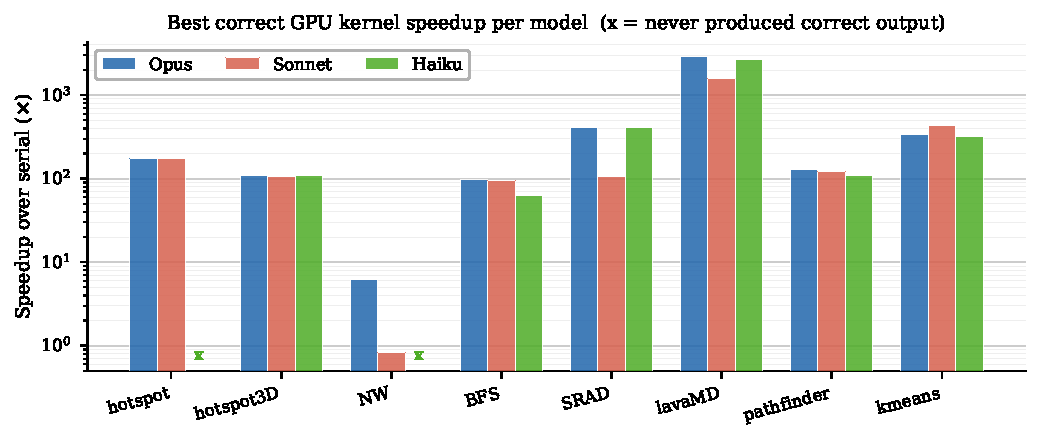
\includegraphics[width=\columnwidth]{fig1_speedup.pdf}
  \caption{Best correct GPU kernel speedup (log scale) per model per benchmark.
           Benchmarks on the left (hotspot, hotspot3D) are memory-bound: all
           models converge to the same ceiling. Benchmarks in the middle--right
           (SRAD, lavaMD, kmeans) are compute-bound: models diverge.
           NW Sonnet's best correct version is its Phase-1 port at $0.8\times$
           (launch overhead dominates this small wavefront; its Phase-2 tiling
           attempts were all incorrect). $\times$~=~never produced correct output.}
  \label{fig:speedup}
\end{figure}

\subsection{Phase~1 Correctness}

We first clarify what counts as a \emph{failure}. A Phase~1 error is not
terminal: the model still receives its Phase~2 rounds to recover. We therefore
reserve the term failure for a benchmark on which a model produces no correct
version at \emph{any} stage---neither its Phase~1 port nor any of its subsequent
Phase~2 rounds.

Phase~1 correctness already reveals a model-tier difference. Opus produced
correct Phase~1 code on 7 of 8 benchmarks, failing only SRAD (a copy-paste
error in the stencil conductance lookup); Sonnet likewise failed only SRAD in
Phase~1. Neither is a true failure---both recovered on SRAD in Phase~2. Haiku,
by contrast, stumbled in Phase~1 on hotspot (incorrect ping-pong buffer
selection) and NW (a host function called from device context), and---unlike
Opus and Sonnet on SRAD---never recovered: it ran all subsequent Phase~2 rounds
on both benchmarks but produced a fresh distinct bug each round, never reaching
a correct version. These are the only two genuine failures in the study.

On the three benchmarks where all models had a correct Phase~1 (lavaMD,
pathfinder, kmeans), the naive speedups track the benchmark's parallelism, not
the model tier ($\sim$1600$\times$ for lavaMD, 70--80$\times$ for kmeans,
33--94$\times$ for pathfinder); the within-benchmark spread reflects generation
variance in block-size and loop-structure choices rather than capability.
Phase~2 then adds a benchmark-dependent multiplier ($\sim$5$\times$ kmeans,
up to 3$\times$ pathfinder, 1.9$\times$ lavaMD), so the clearest model
differentiation emerges in Phase~2, not Phase~1.

\subsection{Phase~2 Optimization Gains}

\textbf{Compute-bound benchmarks (lavaMD, SRAD).}
Phase~2 produces the largest gains here. On lavaMD, Opus improved from
1.30\,ms to 0.70\,ms ($1.9\times$) via shared-memory float4 neighbor staging;
Haiku reached 0.75\,ms by a similar approach. Sonnet's Phase~2 rounds all
produced incorrect output (numerical mismatches), leaving it at the Phase~1
result (1.29\,ms).
On SRAD, Haiku is the only model with a correct Phase~1 (240\,ms); it then
improved $15\times$ to 16.1\,ms via shared-memory reduction and kernel fusion.
Opus Phase~1 was incorrect but recovered in Phase~2 to 16.1\,ms. Sonnet
recovered more slowly, reaching 62\,ms.

\textbf{Memory/transfer-bound benchmarks (hotspot, hotspot3D, BFS).}
Phase~2 yields no significant gain on any of these. The hotspot 5-point stencil
is largely cache-served on Ampere's 4\,MB L2, so candidates reach 33--34\,ms
regardless of strategy; hotspot3D saturates at 6.5--6.7\,ms; and BFS is dominated
by the host-to-device transfer (4.3\,ms), with the kernel (0.8--1.2\,ms) near the
bandwidth ceiling. All models reach the same ceiling and tier has no effect.

\textbf{Wavefront and DP benchmarks (NW, pathfinder).}
On pathfinder (row-parallel DP), all three models reach similar results
(1.04--1.21\,ms) after Phase~2, showing that this benchmark's optimization
ceiling is accessible to all tiers.
NW (wavefront DP) shows the starkest model-tier difference: Opus found the
anti-diagonal tiling strategy in Phase~2 (10.98\,ms\,$\to$\,1.46\,ms, $7.5\times$);
Sonnet attempted four Phase~2 rounds but all produced incorrect output,
leaving it at 11.0\,ms---slower than serial (0.8$\times$) due to GPU launch
overhead dominating a small-input wavefront. Haiku never produced a correct
version: its Phase~1 failed to compile and all four Phase~2 rounds were
incorrect as well.

\textbf{Embarrassingly parallel benchmark (kmeans).}
The assign step is data-parallel over points, so all three models produce a
correct naive Phase~1 port, but at a modest $70$--$80\times$---the naive
kernel reloads the centroid array from global memory for every point. Phase~2
then delivers a large, real gain: placing the small centroid array in constant
memory removes those redundant loads, taking Sonnet to 0.40\,ms (423$\times$)
and Opus to 0.50\,ms (337$\times$)---roughly a $5\times$ improvement over
Phase~1. All models produce correct output with exact integer match throughout,
as the oracle design isolates the GPU assign step from the CPU update step.

\begin{figure*}[t]
  \centering
  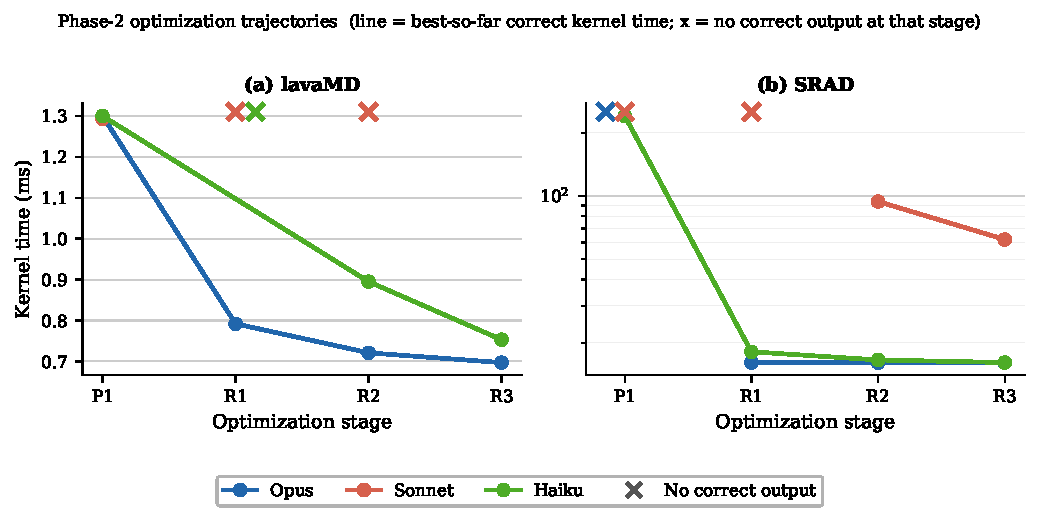
\includegraphics[width=\textwidth]{fig2_trajectory.pdf}
  \caption{Phase-2 optimization trajectories for lavaMD and SRAD.
           Each line shows the best correct kernel time achieved so far;
           a gap at a stage means the model produced no correct output there.
           \textbf{(a)}~lavaMD: Opus improves monotonically across all three
           rounds; Haiku's line resumes at R2 after a gap at R1 (incorrect
           attempt, reverted); Sonnet stops at Phase~1---both R1 and R2 failed.
           \textbf{(b)}~SRAD (log scale): Haiku is the only model with a
           correct Phase~1 (240\,ms) and improves monotonically to 16\,ms;
           Opus has a gap at Phase~1 but immediately reaches 16\,ms at R1;
           Sonnet's line starts only at R2 (94\,ms) after two failed stages.}
  \label{fig:trajectory}
\end{figure*}

%------------------------------------------------------------------------------
\section{Discussion and Analysis}
\label{sec:discussion}

\subsection{Root-cause Analysis of Correctness Bugs}

We dissect the concrete bugs each model introduced. We distinguish two
categories. \emph{Terminal failures} are bugs the model never recovered from
at any stage---these occur only on Haiku (hotspot, NW) and explain
the two ``---'' entries in Table~\ref{tab:results}. \emph{Recoverable bugs} are
errors in a single stage that the model either corrected in a later round or
fell back from to an earlier correct version; these do not cost the benchmark
but are equally informative about each model's characteristic error modes.

\medskip\noindent\textit{Terminal failures (Haiku).}

\textbf{Haiku on hotspot (Phase~1, 1,047,906/1,048,576 mismatches).}
The ping-pong buffer selection uses the parity of the iteration count to infer
which buffer holds the final result: it assigns the result-side buffer when the
iteration count is odd, and the temp-side buffer when even.
However, the kernel loop swaps the live-data pointer each step, so after
$n$ swaps the result resides in whichever pointer the loop variable currently
points to---not a simple function of $n \bmod 2$. For 1000 iterations (even),
the code returns the original input buffer, outputting the initial temperature
field. This is a \emph{pointer-aliasing confusion}: Haiku correctly understood
the ping-pong pattern structurally but failed to track which
variable held the current reference after the swap.

\textbf{Haiku on NW (Phase~1, build error).}
The helper function \texttt{maximum(int,int,int)} was declared as a plain
\texttt{static} function (host-only by default), then called inside a
\texttt{\_\_global\_\_} kernel; the compiler rejected the invocation with a
host/device qualification error.
The fix is a single \texttt{\_\_device\_\_} qualifier. Both Haiku failures are
rooted in \emph{CUDA execution-model details}---not algorithmic
misunderstanding---suggesting the model has internalized the algorithm but
under-represents host/device distinctions. In both cases the subsequent Phase~2
rounds introduced a fresh, distinct bug each round rather than fixing the
original, so Haiku never reached a correct version.

\medskip\noindent\textit{Recoverable bugs (Sonnet, Opus).}

\textbf{Sonnet on NW (Phase~2, all rounds, $>$4M mismatches).}
Sonnet kept its correct Phase~1 port (11.0\,ms) as a fallback, but every Phase~2
attempt was incorrect: it replaced the reference sequence generation
(\texttt{srand(7)}, integer indices 1--10) with its own character-alphabet
scheme and a custom score map, so the \texttt{reference[]} table holds
incompatible values before the DP even begins. This pattern---\emph{substituting
a semantically equivalent but format-incompatible implementation}---recurs across
Sonnet's Phase~2 regressions: it gets the algorithm right but rewrites supporting
code in a way that breaks the oracle contract.

\textbf{Sonnet on lavaMD (Phase~2 r1, 170k mismatches).}
The inner force loop omits the self-interaction guard (\texttt{if (j != i)})
present in the serial reference when processing the home box, so each particle
adds its own contribution to its own force accumulator. The error is subtle---it
does not crash and most mismatches are small---but the oracle catches it
(max relative error 0.27); Sonnet again fell back to its correct Phase~1 port.

\textbf{Opus on SRAD (Phase~1, 4,665/4,194,304 mismatches).}
In the stencil update kernel, the west-direction conductance coefficient is
read using the current-cell index instead of the west-neighbor index
\texttt{c[i*cols + (j-1)]}---a copy-paste error from the north-direction line
above it. Only 4,665 cells are affected---those where the west and current
conductances differ enough to exceed the tolerance---making this a
\emph{near-miss} that a less strict oracle would not detect. Opus corrected it
in the first Phase~2 round, recovering to 16.1\,ms (396$\times$), so SRAD is not
a failure for Opus despite the Phase~1 stumble.

\subsection{Model Optimization Strategies}

\textbf{Opus} applies incremental, targeted optimizations: each Phase~2 round
makes one focused change (e.g., shared-memory \texttt{float4} partner-staging in
lavaMD r1, then occupancy tuning via \texttt{\_\_launch\_\_bounds\_\_} in
r2--r3; see Appendix~D), yielding monotone improvement across all three rounds.
This conservative strategy rarely regresses but can miss more aggressive
reorganizations that require disrupting the overall kernel structure.

\textbf{Sonnet} tends to restructure aggressively: it identifies high-level
optimization targets correctly (tiling strategy for NW, loop restructuring for
lavaMD) but frequently introduces subtle contract violations in the process---
changed sequence generation, missing boundary checks, altered output ordering.
When it avoids these pitfalls, it achieves the best result on kmeans
(0.40\,ms vs.\ Opus's 0.50\,ms), though this margin is within blind-generation
variance (Sec.~\ref{sec:threats}).

\textbf{Haiku} improves steadily where the parallelism is straightforward
(SRAD 240$\to$16.1\,ms over three monotone rounds; lavaMD 0.75\,ms, within 7\%
of Opus), but its correctness is fragile on benchmarks that require careful
tracking of execution-model state (hotspot ping-pong, NW wavefront), suggesting
a less robust CUDA mental model for complex control patterns.

\subsection{Benchmark Type Dominates Model Tier}

In our single-generation study, the benchmark's parallelism structure is a
better guide to the outcome than the model tier. On
\textbf{memory/transfer-bound} benchmarks (hotspot, hotspot3D, BFS),
every model that produces correct code plateaus at the same hardware ceiling
regardless of optimization strategy: hotspot converges to 33--34\,ms
(bandwidth-limited 5-point stencil), hotspot3D to 6.5--6.7\,ms, and BFS to
0.8--1.2\,ms kernel time with the one-time HtoD transfer (4.3\,ms) dominating
total runtime.

On \textbf{compute-bound} benchmarks (lavaMD, SRAD, kmeans), all three models
achieve significant speedups and the ranking is not tier-ordered: on SRAD the
lightweight Haiku ties the frontier Opus (both 16.1\,ms) while Sonnet trails far
behind at 62\,ms; Sonnet wins kmeans (0.40\,ms vs.\ Opus 0.50\,ms vs.\ Haiku
0.53\,ms); and Opus wins lavaMD (0.70\,ms vs.\ Haiku 0.75\,ms). The deciding
factor is which optimization strategy the model lands, not its tier. We stress,
however, that these compute-bound margins are small---often within 10--25\%---and
fall within the run-to-run variance of blind generation (Sec.~\ref{sec:threats}).
We therefore read them as ``all three models reach the same class of result,''
not as a stable performance ranking.

\textbf{Complex parallel structure} (NW wavefront) shows the clearest
tier effect: Opus derived the anti-diagonal tiling strategy in a single round
(10.98$\to$1.46\,ms, $7.5\times$), whereas Sonnet's four attempts all produced
fundamentally incorrect kernels (it fell back to its correct but launch-bound
Phase~1 port) and Haiku never reached a correct version at all.

\subsection{Comparison to the Rodinia Hand-Tuned Reference}

To calibrate against human expertise, we built the \emph{original} Rodinia CUDA
kernels and timed them on the identical workloads and metric
(Table~\ref{tab:results}). Wherever a fair comparison is possible, the best AI
kernel \emph{matches or exceeds} the hand-tuned reference: NW ties (1.46 vs.\
1.42\,ms), lavaMD and pathfinder are $\sim$1.3$\times$ faster, BFS is comparable
at the transfer ceiling, and hotspot is $\sim$5$\times$ faster (33.7 vs.\
160\,ms)---Rodinia's pyramidal temporal-blocking, tuned for 2009-era caches, is
counterproductive on Ampere's 4\,MB L2. The reference also shows its age
elsewhere: the stock SRAD kernels fault (out-of-bounds) under modern CUDA, and
lavaMD ships in fp64 (71.7\,ms here until converted to fp32). We do not claim the
models out-engineer human experts; rather, a frontier LLM targeting
\emph{current} hardware from a serial specification reliably reaches---and
sometimes surpasses---the performance class of a decade-old expert
implementation.

\subsection{Harness Design Lessons}

\textbf{Revert-to-best policy.}
On lavaMD, Haiku's Phase~2 Round~1 was incorrect (191,906/400,000
mismatches). The revert-to-best policy discarded this result and
re-issued Round~2 from the Phase~1 baseline (1.30\,ms).
It recovered to 0.89\,ms and then 0.75\,ms (Fig.~\ref{fig:trajectory}a). Without
reversion, an incorrect intermediate would corrupt the context fed to later
rounds; the policy matters most for the models with higher Phase~2 regression
rates (Sonnet, Haiku).

\textbf{Diagnoser premature-stop suppression.}
The improvement guard blocks a convergence call while per-round gains exceed 5\%.
On lavaMD, Opus improved 1.30\,$\to$\,0.79\,$\to$\,0.72\,$\to$\,0.70\,ms (gains
39\%, 9\%, 3\%); without the guard a conservative diagnoser could have stopped at
0.79\,ms after the first gain, forgoing the further 12\% improvement to 0.70\,ms.

\subsection{Threats to Validity}
\label{sec:threats}

\textbf{Single generation and variance.} Each (model, benchmark, stage) is
generated once; we never resample. Blind generation is stochastic in both
correctness and quality, so a single draw cannot separate capability from
sampling luck---on the two benchmarks we did rerun, both the BFS and SRAD
winners changed and SRAD's full ordering inverted. For the sub-millisecond
ceiling-bound kernels (BFS, hotspot, hotspot3D), run-to-run timing noise is
moreover comparable to the inter-model gaps. We therefore treat compute-bound
performance \emph{rankings} as one sample and rely on the stable qualitative
findings (ceiling convergence, correctness modes).

\textbf{Training-data exposure.} Rodinia long predates these models, so canonical
CUDA solutions were very likely in their training data; our write-only harness
blocks reading a reference at run time but cannot guarantee the model has not
internalized one. We thus measure reproduction-and-tuning of a known pattern,
not parallelization of a novel algorithm.

\textbf{Spec hints and oracle.} The Phase~1 specification names likely
optimization opportunities (e.g., constant memory for the kmeans centroids), so
some Phase~2 wins confirm a hinted direction. Float tolerances (rtol/atol
$10^{-3}$/$10^{-2}$ for lavaMD, $10^{-4}$/$10^{-4}$ otherwise) are tight enough
that the two near-miss bugs would slip past a looser oracle.

%------------------------------------------------------------------------------
\section{Conclusion}

Across eight Rodinia CUDA benchmarks, the benchmark's parallelism structure is
a stronger guide to the outcome than the model tier: all models converge to the
same ceiling on memory-bound workloads, while compute-bound benchmarks expose
differences in correctness and optimization depth. Correctness is the clearest
differentiator---Opus is correct on all eight; Sonnet regresses during
aggressive Phase~2 restructuring; and Haiku fails specifically where careful
CUDA execution-model reasoning is needed (ping-pong buffers, host/device
qualification). Where all models succeed, AI-generated CUDA reaches large
speedups (lavaMD: 0.70\,ms, 2891$\times$) and, on every benchmark we could
compare directly, matches or exceeds the original Rodinia hand-tuned kernel.
The chief limitation (Sec.~\ref{sec:threats}) is the single-generation protocol:
compute-bound margins fall within blind-generation variance, so we report them
as a class of result, not a ranking. Whether repeated sampling closes the
Haiku--Opus reliability gap remains open for future work.

%------------------------------------------------------------------------------
\begin{thebibliography}{00}
\bibitem{che2009rodinia}
S.~Che et al., ``Rodinia: A benchmark suite for heterogeneous computing,''
\emph{IISWC}, 2009.

\bibitem{chen2021codex}
M.~Chen et al., ``Evaluating large language models trained on code,''
\emph{arXiv:2107.03374}, 2021.

\bibitem{gpa2021}
K.~Zhou, X.~Meng, R.~Sai, and J.~Mellor-Crummey, ``GPA: A GPU performance
advisor based on instruction sampling,'' \emph{CGO}, 2021.

\bibitem{rodinia2010}
S.~Che et al., ``A characterization of the Rodinia benchmark suite with
comparison to contemporary CMP workloads,'' \emph{IISWC}, 2010.
\end{thebibliography}

\xdef\mainbodyendpage{\thepage}

\clearpage
%==============================================================================
%  APPENDIX
%==============================================================================
\appendices

\section{Phase 1 System Prompt (Generation Agent)}
\begin{lstlisting}
You are a CUDA code generation agent. You write complete, compilable
CUDA source files. You have access to Write (to write files) only.
You cannot read any files in the repository.
You write exactly one .cu file per invocation.
\end{lstlisting}

\section{Phase 1 Input Prompt Structure}
\begin{lstlisting}
PHASE 1 - BASIC PARALLELIZATION ONLY. Identify the parallelism
in the serial code and write a correct, straightforward CUDA port.
Use GLOBAL memory only. Do NOT use shared memory, tiling,
temporal/blocking, or other hardware-specific optimizations.
Match the EXACT CLI and output format.

Write the full .cu to: <path>

=== ALGORITHM SPEC ===
<ALGORITHM.md contents>

=== CLI/IO ===
<one-paragraph CLI restatement>

=== SERIAL REFERENCE ===
<serial .c full source>
\end{lstlisting}

\section{Phase 2 Diagnoser Prompt Structure}
\begin{lstlisting}
You are reviewing a CUDA candidate for benchmark "<bm>".
Read the candidate file <path> (use Read). This is the BEST
CORRECT version so far (<stage>, kernel <ms> ms, <speedup>x).
Its measured evaluation: <eval JSON with kernel_ms, htod_ms,
dtoh_ms, kernel_breakdown, mismatches, error_excerpt>

[If last round regressed:]
IMPORTANT: your most recent attempt (<stage>) is NOT this file.
It [was correct but SLOWER / was INCORRECT / FAILED TO BUILD].
Do NOT repeat that change.

Phase-2 goal: minimize GPU kernel time; hardware optimizations
(shared memory, tiling, coalescing, occupancy, fewer launches)
are ALLOWED. Do NOT read any reference implementation.

Return: prev_code = full file contents; diagnosis = actionable
feedback; stop = true only if no >5% improvement expected.
\end{lstlisting}

\section{Case Study: Opus's lavaMD Optimization}

To make the diagnose--regenerate loop concrete, we trace how Opus reached the
best lavaMD result (0.70\,ms, 2891$\times$) over its four stages.

\textbf{Phase~1 (1.30\,ms).} A correct one-thread-per-particle port: each thread
loops over its home box and the 26 neighbouring boxes, reading every partner
particle straight from global memory.

\textbf{Round~1 (0.79\,ms, $-$39\%).} The diagnoser identified the inner
force-sum loop as global-memory-bound---every home thread re-reads each partner
from DRAM---and suggested shared-memory staging. Opus loaded each partner record
$(x,y,z,v)$ once per block into a packed \texttt{\_\_shared\_\_ float4} tile, so
the hot loop issues a single 128-bit shared load per partner instead of four
separate global reads. This one change is the dominant win.

\textbf{Round~2 (0.72\,ms, $-$9\%).} With the kernel now occupancy-bound, Opus
added \texttt{\_\_launch\_\_bounds\_\_} so the compiler could fit more
thread blocks per SM.

\textbf{Round~3 (0.70\,ms, $-$3\%).} A final occupancy tune
(\texttt{\_\_launch\_\_bounds\_\_(100,8)}). The gain fell below the 5\%
threshold, so the loop terminated---the intended convergence behavior.

\vspace{0.5em}
\noindent Repository: \url{https://github.com/KappaBarbarosa/gpu-rodinia}

\end{document}
